\subsection{Ca sử dụng xem danh sách khuôn mặt}

Người dùng xem danh sách các khuôn mặt được hệ thống phát hiện trong ảnh. Khi nhận được yêu cầu từ người dùng, hệ thống sẽ lấy dữ liệu khuôn mặt từ ảnh và phân loại chúng thành các nhóm khuôn mặt. Nếu có những nhóm khuôn mặt đã được tạo trước đó thì hệ thống sẽ so sánh nhóm khuôn mặt mới với nhóm khuôn mặt cũ. Nếu phù hợp thì nhóm mới sẽ thay thế nhóm cũ.  

Mô tả chi tiết cho ca sử dụng xem danh sách khuôn mặt được thể hiện ở Bảng \ref{tab:view-face-usecase} dưới đây. Kèm theo là Bảng \ref{tab:view-face-usecase-activity} về biểu đồ hoạt động, quan hệ và Hình \ref{fig:3-3-10-sequence-diagram} về biểu đồ tuần tự của ca sử dụng này. 

\noindent 
\begin{table}[H]
\centering
\caption{Mô tả chi tiết ca sử dụng xem danh sách khuôn mặt}
\label{tab:view-face-usecase}
\begin{tabularx}{\linewidth}{| l | X |} 
\hline 
\textbf{Mô tả} & Người dùng muốn xem các danh sách khuôn mặt xuất hiện trong các bức ảnh tải lên. \\
\hline 
\textbf{Luồng cơ bản} & 1. Người dùng bấm vào ô khám phá khuôn mặt. \newline
                       2. Hệ thống lấy dữ liệu những khuôn mặt trong ảnh người dùng. \newline
                       3. Hệ thống lấy dữ liệu nhóm khuôn mặt đã được tạo trước đó. \newline
                       4. Hệ thống thực hiện phân loại và so sánh nhóm khuôn mặt mới với nhóm khuôn mặt cũ. \newline
                       5. Hệ thống hiển thị danh sách các khuôn mặt và tên gọi (nếu có). \\
\hline
\textbf{Luồng thay thế} & 2a. Nếu có những nhóm khuôn mặt có sẵn thì hệ thống so sánh nhóm mới với nhóm cũ. Và sau đó nhóm mới sẽ thay thế nhóm cũ nếu phù hợp. \\
\hline
\textbf{Tiền điều kiện} & - Người dùng đã đăng nhập vào hệ thống. \newline
                           - Hệ thống đã phân loại khuôn mặt trong ảnh. \\
\textbf{Hậu điều kiện} & - Hệ thống hiển thị trạng thái và tiến độ tạo video theo thời gian thực. \newline
                         - Người dùng quay về màn hình danh sách video để theo dõi trạng thái video đã tạo. \\
\hline 
\textbf{Yêu cầu phi chức năng} & -Hệ thống xử lý nhóm khuôn mặt không quá 20s. \\
\hline 
\end{tabularx}
\end{table}

\vspace{0.8cm}

\noindent 
\begin{table}[H]
\centering
\caption{Biểu đồ hoạt động và quan hệ ca sử dụng xem danh sách khuôn mặt}
\label{tab:view-face-usecase-activity}
\begin{tabular}{| c | c |}
    \hline
    \textbf{Biểu đồ hoạt động} & \textbf{Quan hệ} \\ 
    \hline
    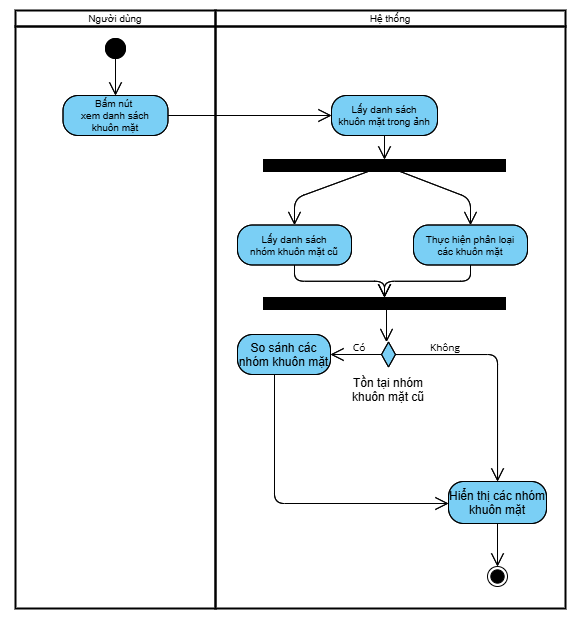
\includegraphics[width=0.6\linewidth]{figures/c3/3-3-10-activity-diagram.png} 
    &  
    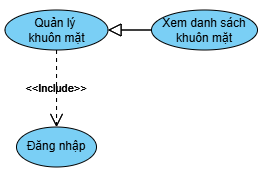
\includegraphics[width=0.35\linewidth]{figures/c3/3-3-10-relationship.png} \\ 
    \hline
\end{tabular}
\end{table}

\begin{figure}[H]
    \centering  
    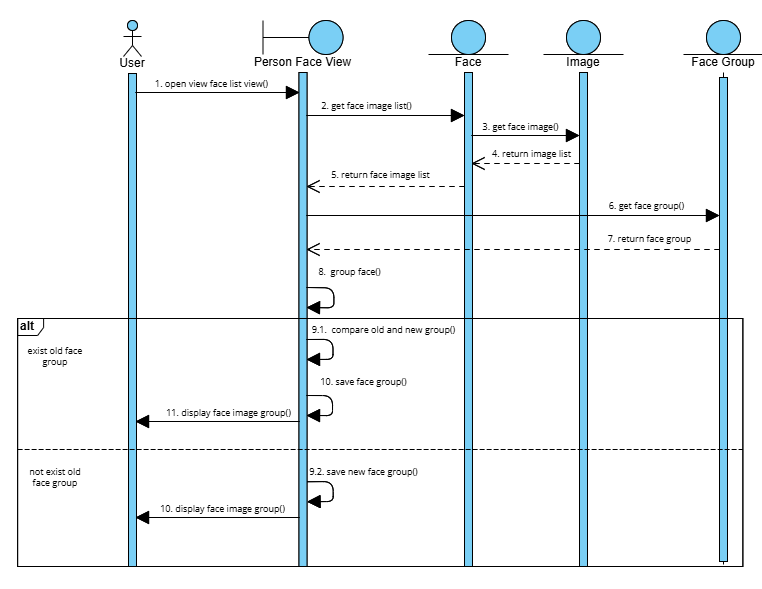
\includegraphics[width=1\textwidth]{figures/c3/3-3-10-sequence-diagram.png}
    \caption{Biểu đồ tuần tự ca sử dụng xem danh sách khuôn mặt.}
    \label{fig:3-3-10-sequence-diagram}
\end{figure}